\section{Crossing Fiber Tractography with Reduced Measurement Uncertainty}

\subsection{Probabilistic Streamline-Based Tractography}
\begin{figure*}[h]
	\centering
	\begin{subfigure}[b]{0.45\linewidth}
		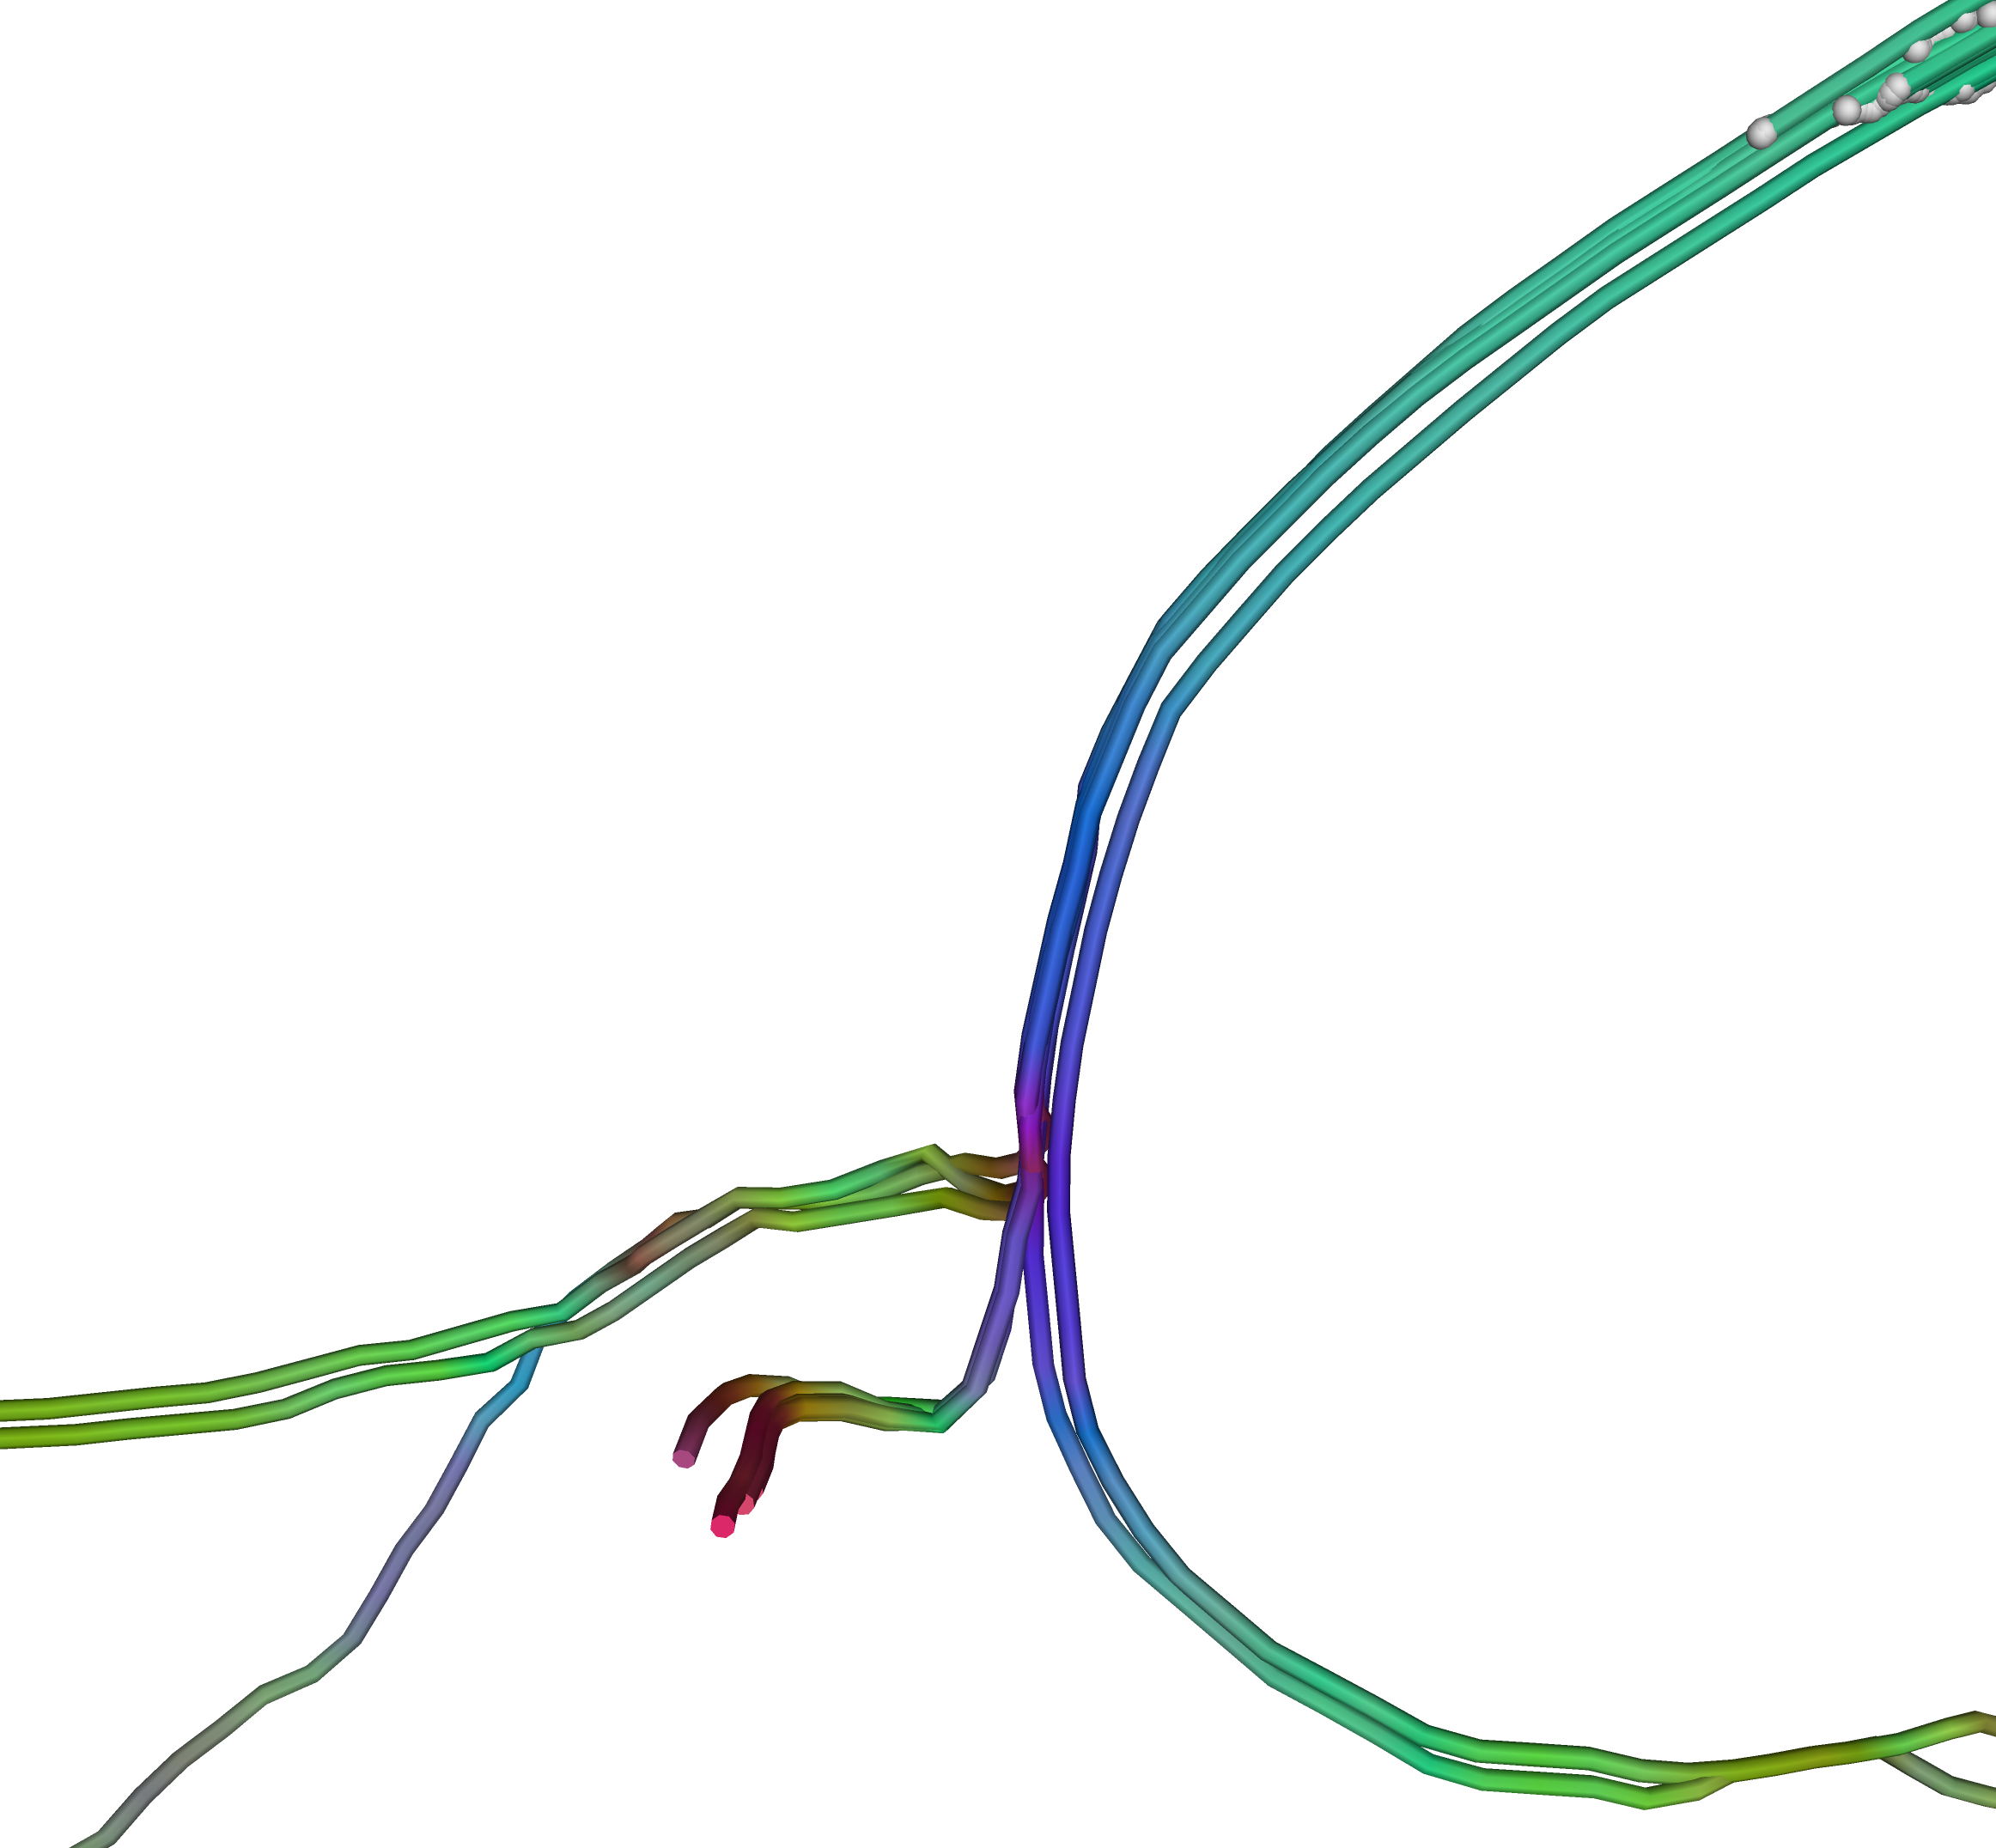
\includegraphics[width=\linewidth]{FACT}
		\caption{Nearest neighbor interpolation}
	\end{subfigure}
	\begin{subfigure}[b]{0.45\linewidth}
		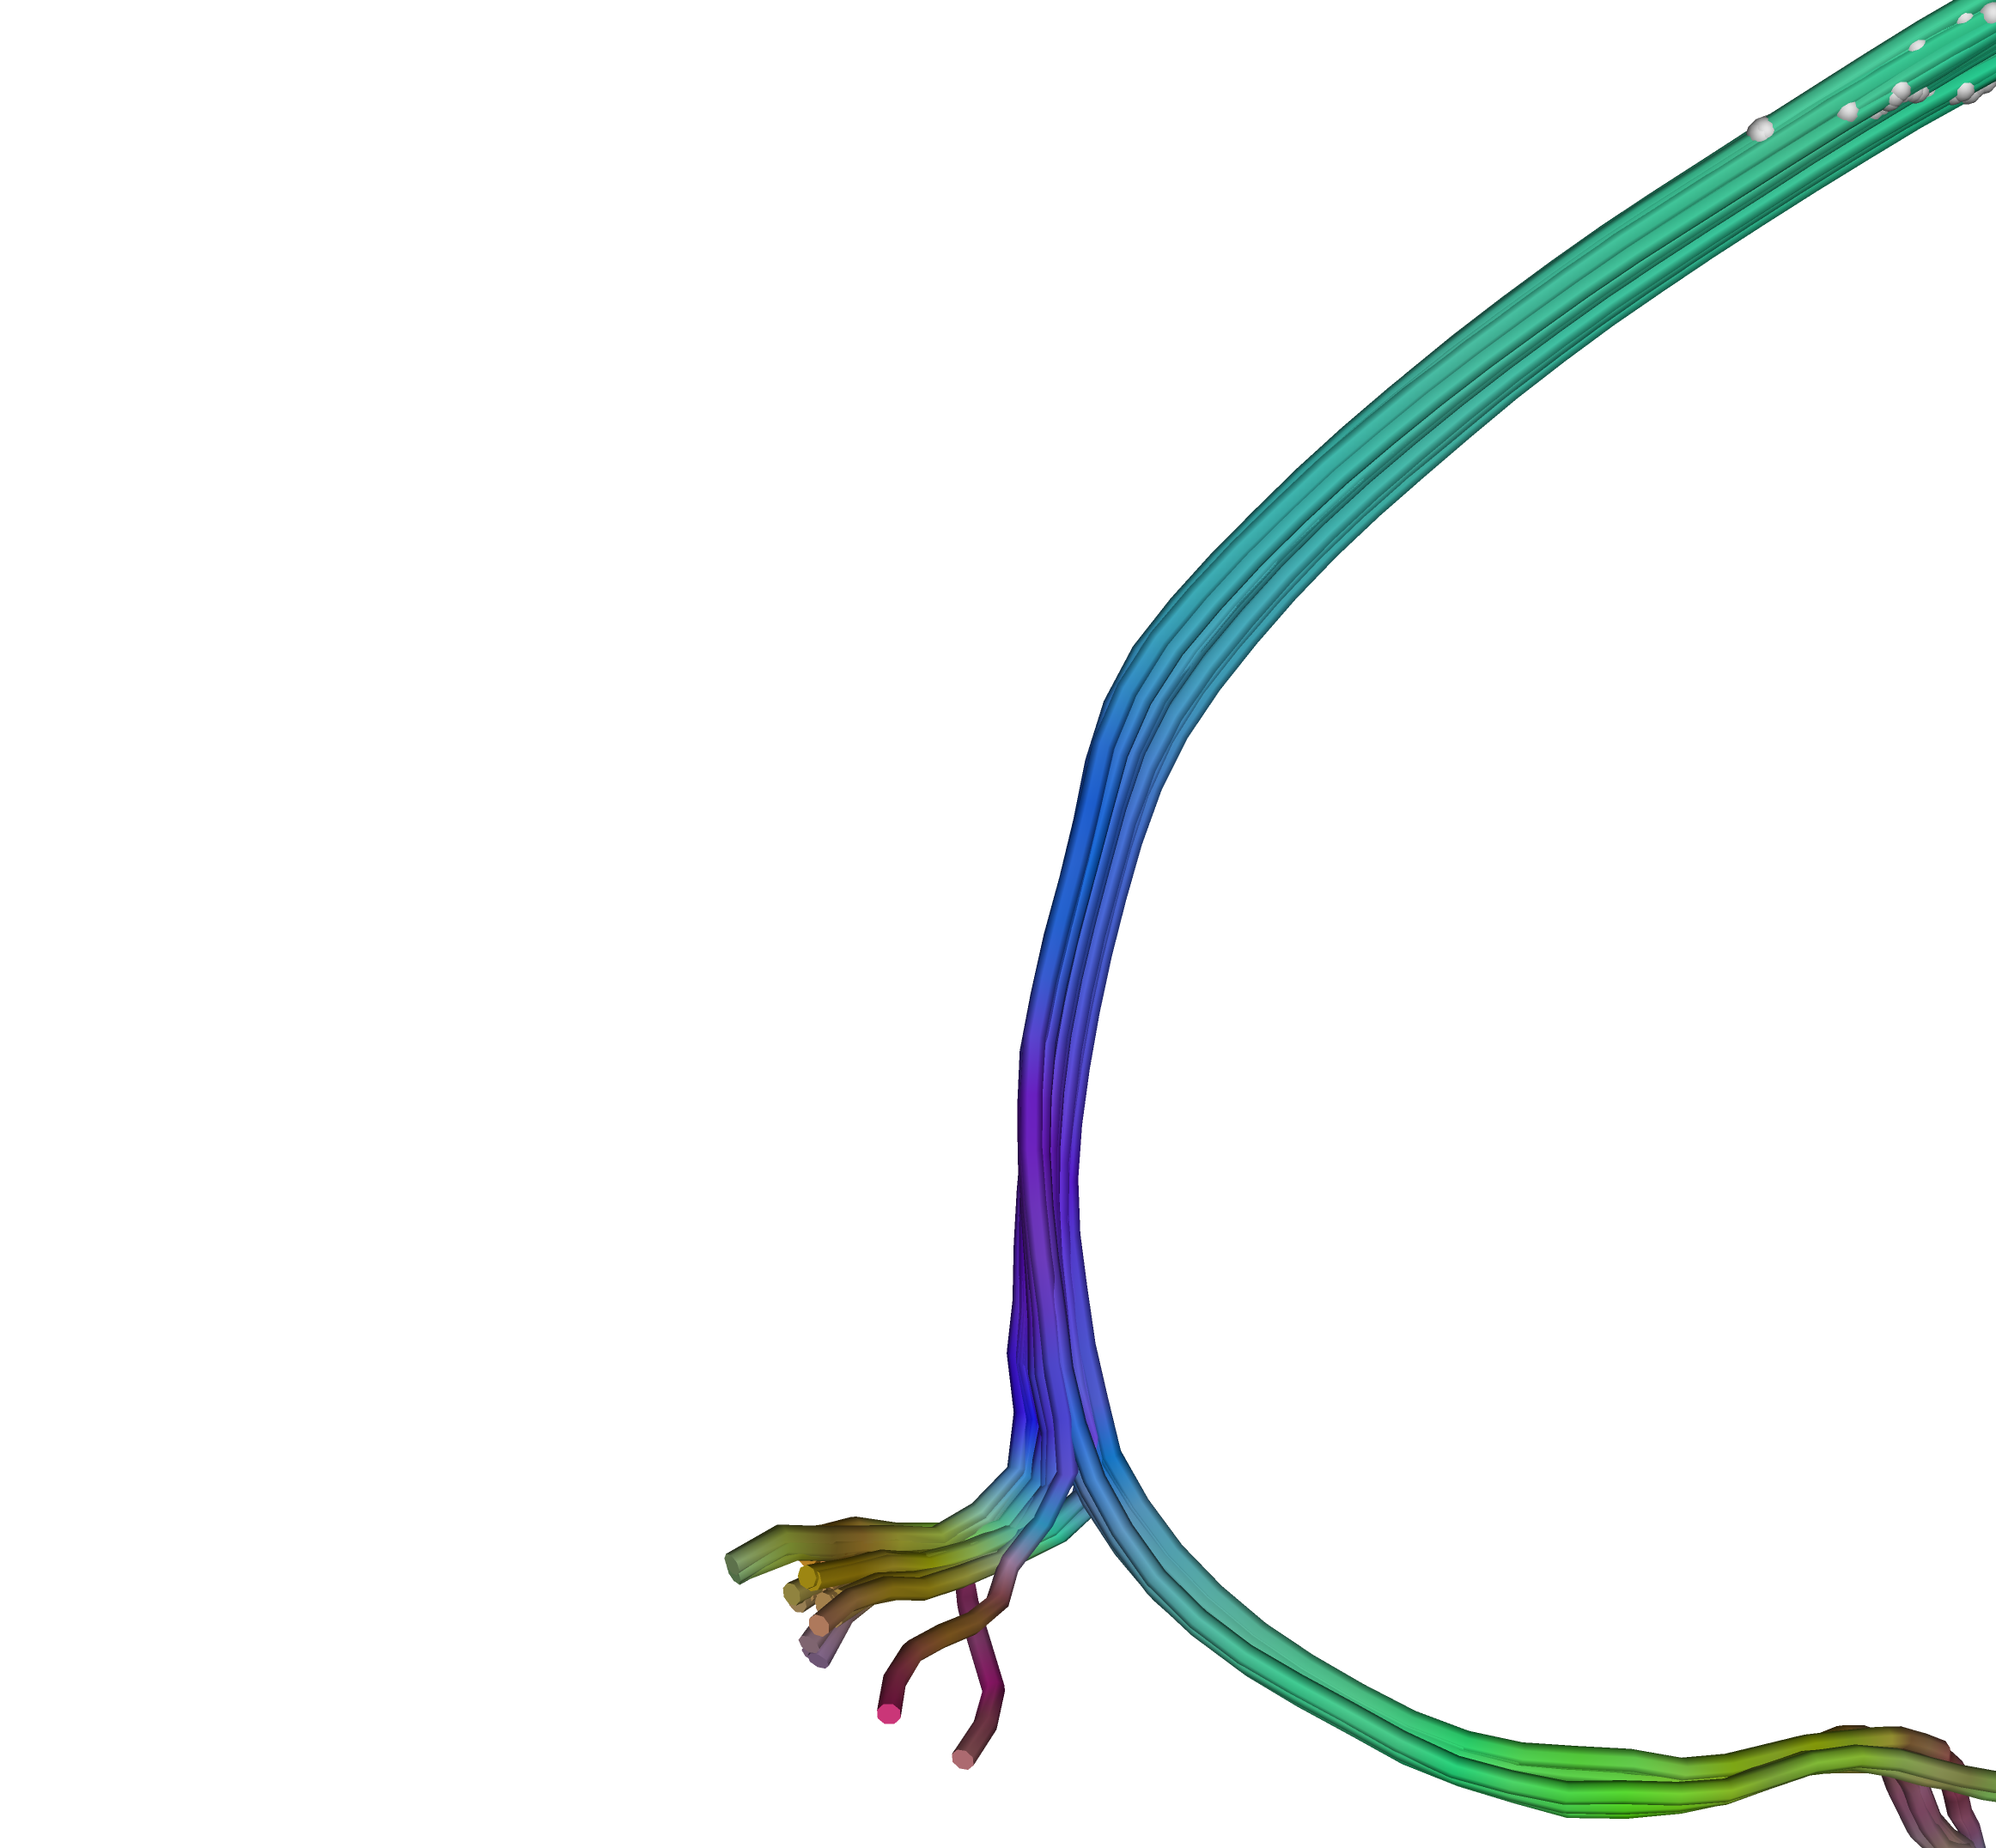
\includegraphics[width=\linewidth]{Trilinear}
		\caption{Trilinear interpolation}
	\end{subfigure}
	\caption{Comparison of nearest neighbor interpolation and trilinear
	interpolation in the front part of the cingulum. Seedpoints are in the
upper right corner.}

	\label{fig:interpolation-comparison}
\end{figure*}
Within this work a probabilistic streamline-based approach is used. For a given
seed point, the streamline grows iteratively in both directions using Euler
integration. Since neither the seed point nor any other point of the streamline
lies on a grid point, we interpolate the current position trilinearly. Therefore,
we have to solve a matching problem first, since we have to decide which
directions belong together to apply the trilinear interpolation. Since we assume
smoothness between the voxels we use the three directions, from the last
interpolation step as group means $\bar{\mathbf{v}}_i$, $i \in \left\{ 1\dots 3 
\right\}$. Now we fit each vertex to the group means such
that 
\begin{align}
	\text{Sym} \left( r  \right) & \rightarrow \mathbb{R}_+ \\ 
	Z & \mapsto \sum \| \sgn \left( \langle \mathbf{v}_{Z \left( i \right)}
	, \bar{\mathbf{v}}_i \rangle  \right) \mathbf{v}_{Z \left( i \right)} -
\bar{\mathbf{v}}_i
	\|
\end{align}
is minimized. We only update the group means if a group mean is not defined.
Then we solve the above minimization problem and assign the direction as new
group mean. Afterwards, we rerun the minimization for all vertices. This is done,
to reduce the time consumption drastically. Further, the local optimal
configuration is cached. Using this, we only have to calculate the assignments
once for each voxel which we are tracking through. 
To initialize the trilinear interpolation, we take the directions of the nearest voxel as group means.
Given the interpolated directions $\mathbf{v}_i$ at the current point, we
reorient them to have a non-negative inner product with the current tracking
direction $\mathbf{w}$. We select one of the $r$ possible directions by the
following probabilistic model.

We assign each unit direction $\mathbf{v}_i$ with the volume fraction
$\lambda_i$ for $i \in \left\{ 1\dots r \right\}$ following the probability
scheme 
\[
	p \left( \mathbf{v}_i \right) \coloneqq \frac{ \mathbb{1}_{\lbrace\theta_i <
		\frac{1}{3} \pi \rbrace} \lambda_i \cos \left( \left( \frac{3}{\sqrt{2
\pi}} \theta_i \right)^2 \right)}{\sum_j \mathbb{1}_{\lbrace\theta_j <
		\frac{1}{3} \pi \rbrace} \lambda_j \cos \left( \left( \frac{3}{\sqrt{2
\pi}} \theta_j \right)^2 \right) }, 
\]
where $\theta_i$ denotes the angle between the possible direction $\mathbf{v}_i$
and the current direction $\mathbf{w}$. 

The proposed probability function assigns angles below 30 degrees almost the
same probability, which coincides with the limited angular resolution of
spherical deconvolution \cite{TOURNIER20071459}. Further, the maximum angle is
restricted to 60 degrees, which coincides with our anatomical knowledge.

This iterative algorithm proceeds until we either reach a region with fractional
anisotropy below $0.3$ or the summed angle over the last $30$ mm is greater than
$130$ degrees. This prevents streamlines to go back and forth. In latter case
the entire streamline gets removed. 

In Fig. \ref{fig:interpolation-comparison} we have visualized the nearest
neighbor interpolation, which was used within the last paper and the trilinear
interpolation which we use from now on. The constrains are set as mentioned
above and to create a better comparison, we used a deterministic approach, which
always follows the direction with the smallest angle compared to the current
direction. It is clearly visible, that the trilinear interpolation is superior
compared to the computational less expensive nearest neighbor interpolation if it comes to
regions with a high curvature. This is due to two main reasons. First of all,
tracking with trilinear interpolation leads to much smoother results and does
not create large angles as the nearest neighbor interpolation does. Secondly,
it is able to reconstruct a larger amount of streamlines within this high
curvature region, because it does not get in conflict with the constrains.

Therefore, we used the trilinear approach within this work and further set the
probabilistic direction selection function more restrictive, i.e. restricting
the maximum angle to 45 degrees instead of 60.  


\subsection{Postprocessing}
While diffusion MRI is in general able to reconstruct large parts of the white
matter tracts, it is also well known that it is suspiscious to reconstruct false
positives, which have to be removed according to anatomic knowledge
\cite{Wakana:2007, MaierHein:2017}. Further, the probabilistic tracking approach
generates outliers with low density, which have to be removed to have a proper
output. 

To avoid false positives, we use inclusion and exclusion regions. All regions
are set carefully for a reference patient according to [hier die quelle].
The remaining patients are linearly registered to the reference patient and the
linear transformation is used to map the regions to the other patients. 
If a streamline intersects with an exclusion region, the whole streamline is
discarded and if a streamline does not intersect with all inclusion regions, it
is discarded as well. 

Further, we create a density map for each streamline
bundle. Therefore, we count the number of streamlines intersecting each voxel.
All streamlines are cut off at the first intersection with a low density
area starting from the seed. The low density threshold is also defined for the
reference patient and then mapped to all other patients according to the seed
ratio.
